% SAMPLE ARTICLE FOR COMBINATORIAL THEORY
%
% CT papers *must* follow this sample file.
% Please, do not erase comments in the head of this sample file as
% they are used to process your file semi-automatically.

\documentclass[12pt]{article}
\usepackage{ct}

% Additional packages not loaded by ct.sty:
\usepackage{cmap}          % correct ToUnicode ligature mapping in PDF text layer
\input{glyphtounicode}
\pdfgentounicode=1
\pdfinfoomitdate=1         % suppress creation/modification timestamps in PDF metadata
\usepackage{booktabs}  % for \toprule/\midrule/\bottomrule in tables
\usepackage{tikz}      % for figure1.tex

% SPECIFICATIONS
\specs{n}{vol (issue)}{year}{}

% DATES
\dateline{April 10, 2026}{TBD}{TBD}

% KEYWORDS
\keywords{Lonely Runner Conjecture, Diophantine approximation, complementary pairs, coupling principle, arithmetic progressions, boundary-set method, $n=11$}

% SUBJECT CODES
\MSC{11J13, 11B75, 52C07, 11K60}

% TITLE
\title{Eleven Lonely Runners: Complementary Pairs and the Coupling Principle}

% AUTHOR AND AFFILIATION
% Removed for double-blind review per CT submission guidelines.
\author[1]{Anonymous}

\affil[1]{%
Anonymous Institution

\email{anonymous@example.com}%
}

\begin{document}

\maketitle

\begin{abstract}

We prove the classical Lonely Runner Conjecture for $n=11$: for any ten distinct positive
real speeds $e_1<\cdots<e_{10}$ there exists $t>0$ with $\|e_i t\|\ge 1/11$ for all $i$.
The proof splits into three cases (bounded ratio, irrational ratio, and the essential
commensurable large-ratio regime $e_{10}/e_1>10$), with the last handled inside the
isolation window
\[
W_{\mathrm{ref}} = \left[\frac{1}{11e_1},\,\frac{10}{11e_1}\right].
\]
The commensurable case rests on two structural facts: the prime modulus $11$ forces the
runners $2,\ldots,9$ into four \textbf{complementary pairs}, each pair assigned as the primary
coverage responsibility for two slots and leaving $I_9$ unclaimed; and the \textbf{Coupling Principle} (bad intervals form a rigid arithmetic progression) ensures any off-schedule
attempt to cover $I_9$ creates a gap elsewhere.
All 34 explicit rational inequalities are verified with exact arithmetic, and a boundary-set
witness search over $1.1\times 10^9$ random configurations finds zero failures.

\end{abstract}



\section{Introduction}

The classical Lonely Runner Conjecture, introduced by Wills \cite{Wil67} and reformulated by
Cusick \cite{Cus73}, asserts that for any $n$ distinct nonzero real speeds there exists a
time when every moving runner is at distance at least $1/(n+1)$ from the origin. The cases
up to $n=10$ were established over a long sequence of papers: six runners by Bohman and
Holzman \cite{BH01}, seven by Barajas and Serra \cite{BS08}, and the algebraic and flow-obstruction
perspective developed in \cite{BGG+98}; a comprehensive survey of the conjecture's sixty-year
history and its connections to Diophantine approximation and chromatic graph theory is given by
Perarnau and Serra \cite{PS25}. Structural aspects are also surveyed in \cite{Tao18}. The cases
of eight, nine, and ten runners were settled recently \cite{Ros25a,Ros25b,Tra25}, using methods
that become computationally infeasible at $n=11$; the present proof is purely analytic. We prove
the case $n=11$.

\begin{theorem}[Main Theorem]\label{t:11}
For any ten distinct positive real speeds
$e_1<\cdots<e_{10}$, there exists $t>0$ such that
\[
\|e_i t\|\ge \frac{1}{11}\qquad(i=1,\ldots,10).
\]

The proof has three cases.

\end{theorem}
\begin{theorem}[Bounded-Ratio Theorem]\label{t:12}
If $e_{10}/e_1\le 10$, then
\[
t^*=\frac{10}{11e_{10}}
\]
satisfies $\|e_i t^*\|\ge 1/11$ for all $i$.
\end{theorem}

If any ratio $e_i/e_j$ is irrational, a Kronecker closure argument reduces the problem
to nearby commensurable configurations handled by Corollary 7.6. The proof
is in Appendix C.

The remaining case is the commensurable large-ratio regime
\[
\rho := \frac{e_{10}}{e_1} > 10.
\]
That is the only place where real work is needed, and it is the only place where the algebraic
structure of the prime modulus $11$ plays a role. The proof structure is detailed in the sketch below.

\subsection{Proof sketch}

Two cases are dispensed with quickly. If $e_{10}/e_1\le 10$, the time $t^*=10/(11e_{10})$
is a witness for every runner simultaneously; the proof is two lines. If some speed ratio
is irrational, a Kronecker approximation argument produces commensurable configurations
converging to the original, and any witness for a nearby commensurable configuration
lifts to a witness in an open neighbourhood. This reduction uses the commensurable closure
result of Section 7 but is otherwise self-contained; the proof is in Appendix C.

The real work is the commensurable large-ratio case $e_{10}/e_1>10$. The bounded-ratio
witness $t^*$ fails here because $e_1 t^*=10e_1/(11e_{10})<1/11$. There is no single
explicit time that works uniformly, so the proof must handle a continuous parameter space.

\textbf{Complementary pairs.}
The prime modulus $11$ imposes a rigid algebraic structure. At the AP limit $a_j=j$, each
runner $j\in\{2,\ldots,9\}$ has two witness labels $m_j^{\pm}\equiv\pm j^{-1}\pmod{11}$.
Because $11$ is prime, runners $j$ and $11-j$ share the same two labels: they form a
\emph{complementary pair}. The four pairs --- $(2,9)$, $(3,8)$, $(4,7)$, $(5,6)$ --- together
own eight primary slots $I_1,\ldots,I_8$, two per pair. Slot $I_9$ is left unclaimed:
no pair's label corresponds to it.

\emph{Ownership} here means that at the AP limit the pair's witness labels correspond to
that slot's boundaries, and that any perturbative repair of the slot must be borne by the
pair. It does \emph{not} mean the pair covers the slot under all perturbed configurations;
that is exactly what the gap obstruction lemmas in Section 5 resolve.

\textbf{Coupling principle.}
Each runner's bad intervals form a rigid arithmetic progression in time. Moving one
interval to cover a boundary forces the entire chain to shift proportionally. If a runner
covers the unclaimed slot $I_9$ off schedule (not via its designated primary-slot branch),
its primary slot is left partially open. In each case the lemmas identify the specific slot
that opens: for runners whose normalised speed lies \emph{below} their index $j$ (negative sign,
defined formally in Section 2) the primary slot is directly exposed; for runners whose
normalised speed lies \emph{above} their index $j$ (positive sign) a short cascade forces open
a different slot.

\textbf{The gap obstruction lemmas and their closure.}
The three gap obstruction lemmas in Section 5 each handle a specific class of off-schedule
repair:

\begin{itemize}
\item When a negative-sign runner shifts far enough to cover the residual gap in $I_9$, the
  Coupling Principle forces it to overshoot its own primary slot --- the bad interval that
  should close the slot's right boundary has already passed it. (\textbf{Primary Slot Miss, PSM},
  Lemma 5.3.)
\item Runner 3 with positive sign ($\sigma_3=+1$) can reach $I_9$, but covering that gap
  forces a sub-gap in $I_3$. The proof identifies runner 8 as the unique valid repairer by
  checking three cases on the harmonic index $k'$: $k'=0$ candidates lie entirely left of
  $I_3$; $k'=1$ candidates (runners 5 or 6) have their $k=0$ interval starting above
  $I_1[\text{left}]$ (by the sign-range upper bound $a_{j'}<7$), exposing a gap of width
  $\ge 8/385$ at the left edge of $I_1$ and thereby violating the completely blocking
  assumption; $k'=2$ candidates are outside the sign-range box. Runner 8 via $B_{8,2}$ is
  therefore forced, and it must shift upward, leaving $I_8$ short by a computable margin
  of $1/50$. (\textbf{Chain A}, Lemma 5.4.)
\item Runner 4 with positive sign ($\sigma_4=+1$) forces a sub-gap in $I_2$. The $k'=1$
  alternative repairer (runner 8) is excluded: for any $a_8>7$ the slot $I_3$ falls
  entirely in the gap between $B_{8,1}$ and $B_{8,2}$, leaving $\mathrm{GF}(I_3)>0$.
  The only remaining candidate is runner 7, whose forced lower bound $a_7>7$ contradicts
  the upper bound $a_7\le 560/87<7$ needed to close $I_7$. This is an outright
  incompatibility, so $\mathrm{GF}(I_7)>0$. (\textbf{Chain B}, Lemma 5.5.)
\item \textbf{Universal Blocking} (Theorem 5.6) collects these lemmas and shows that every
  plausible filler for the residual right gap in $I_9$ either fails a speed-range
  feasibility check or triggers one of the above.
\end{itemize}

No completely blocking configuration therefore exists in any single pacemaker cycle
inside $W_{\mathrm{ref}}$ (defined formally in Section 2).

\textbf{Shift invariance and the witness.}
The slot boundaries $I_s$ are defined in pacemaker-relative coordinates (defined formally
in Section 2), and all endpoint inequalities in Sections 5 and 6 involve only speed ranges
and slot boundaries --- not the absolute cycle index $m$. The static-core argument is
therefore shift-invariant: it propagates unchanged to every complete pacemaker cycle
inside $W_{\mathrm{ref}}$. Since $W_{\mathrm{ref}}$ contains at least one complete cycle
whenever $a_1<1$, a witness exists.

\textbf{Organisation.} Section 2 fixes notation. Section 3 dispenses with the bounded-ratio
and irrational-ratio cases. Section 4 establishes the algebraic skeleton: Complementary
Pairs and the Coupling Principle. Section 5 develops the three gap obstruction lemmas
(PSM, Chain A, Chain B), then assembles them into Universal Blocking. Section 6 applies
Universal Blocking to every sign class --- this is the \emph{single-cycle analysis}. Section 7
shows the single-cycle analysis is shift-invariant and propagates it across every complete
pacemaker cycle in $W_{\mathrm{ref}}$. Section 8 assembles the three cases. Appendices A--C
supply interval arithmetic, computational corroboration, and the irrational-case reduction.



\section{Setup and Notation}

Throughout, $\|x\| := \min(\{x\}, 1-\{x\})$ denotes the distance from $x$ to the nearest
integer, where $\{x\}=x-\lfloor x\rfloor$ is the fractional part.

Fix $n=11$ throughout. For a speed vector $e_1<\cdots<e_{10}$, normalise by setting
\[
a_i := \frac{10e_i}{e_{10}},\qquad a_{10}=10.
\]
Thus $0<a_1<a_2<\cdots<a_9<10$. The classical AP witnesses are
\[
t_m = \frac{m}{11},\qquad m=1,\ldots,10.
\]
For runner $j$ with normalised speed $a_j$, the \textbf{bad intervals} are
\[
B_{j,k}(a_j) = \left[\frac{11k+10}{11a_j},\,\frac{11k+12}{11a_j}\right],\qquad k\ge 0,
\]
with width
\[
|B_{j,k}| = \frac{2}{11a_j},
\]
independent of $k$.

The \textbf{pacemaker slots} in cycle-relative coordinates are
\[
I_s = \left[\frac{11s+1}{110},\,\frac{11s+10}{110}\right],\qquad s=1,\ldots,9.
\]
The $m$th \textbf{pacemaker cycle} is $C_m=\bigl[m/10,\,(m+1)/10\bigr]$, and in absolute
coordinates the slots inside that cycle are
\[
I_s^{(m)} = \left[\frac{11m+11s+1}{110},\,\frac{11m+11s+10}{110}\right].
\]
We call these the pacemaker slots and pacemaker cycles because they are set by the
normalised top speed $a_{10}=10$, which gives a natural period of $1/10$ that paces the
analysis of all other runners inside $W_{\mathrm{ref}}$.

In the large-ratio case $a_1<1$, and we work in the window
\[
W_{\mathrm{ref}} = \left[\frac{1}{11a_1},\,\frac{10}{11a_1}\right].
\]
Runner 1 is isolated throughout $W_{\mathrm{ref}}$ by construction.

For any slot $J$, define its \textbf{good fraction} by
\[
\mathrm{GF}(J) = \frac{|J\setminus\bigcup_{j,k}B_{j,k}|}{|J|}.
\]
The good fraction measures how much of a slot is left uncovered; the proof proceeds by
showing $\mathrm{GF}(I_k)>0$ for some slot $k$ in every completely blocking configuration.
A configuration is \textbf{completely blocking} on a pacemaker cycle if $\mathrm{GF}(I_s^{(m)})=0$
for every $s=1,\ldots,9$; the goal is to show no such configuration exists.

In the static-core analysis we use the \textbf{sign convention}
\begin{align*}
\sigma_j =
  \begin{cases}
    +1, & a_j\in(j,\,j+1),\\
    -1, & a_j\in(j-1,\,j).
  \end{cases}
\end{align*}
The sign of runner $j$ records which half of its feasible speed range it occupies,
determining which bad-interval branch is active and which primary slot boundary is at
risk. Concretely: $\sigma_j=+1$ means $B_{j,0}$ sits to the left of its AP-limit
position, so the primary slot's \emph{right} boundary may be exposed; $\sigma_j=-1$ means
$B_{j,0}$ sits to the right, so the \emph{left} boundary is at risk. These two cases drive
the PSM lemma (Lemma 5.3, negative-sign runners) and the Chain A/B cascades
(Lemmas 5.4--5.5, positive-sign runners) respectively.
We exclude the measure-zero hyperplanes $a_j=j$; boundary cases can be handled by a
limiting argument or direct boundary check and do not affect the contradiction analysis.

The slot comparisons that drive the proof are made in cycle-relative coordinates and are
shift-invariant, which is why we call the analysis in Sections 5 and 6 the \textbf{static core}. The \textbf{cycle index} $m$ labels which pacemaker cycle $C_m$ is under consideration;
shift invariance (Section 7) means $m$ never enters the endpoint arithmetic.

\begin{remark}[Terminology guide]\label{rem:21}
\emph{Pacemaker:} the normalised top speed $a_{10}=10$, which sets the cycle grid with
natural period $1/10$.
\emph{Pacemaker cycle $C_m$:} the time block $[m/10,(m+1)/10]$.
\emph{Cycle index $m$:} which block is under analysis. The analysis is shift-invariant if
the endpoint inequalities hold identically for every $m$, i.e.\ $m$ never enters
the arithmetic.
\emph{Sign $\sigma_j$:} whether runner $j$ operates in the upper ($a_j>j$) or lower
($a_j<j$) half of its feasible speed range.
\emph{Ownership (primary-slot correspondence):} the assignment of primary slot-coverage
responsibility to a runner pair at the AP limit (see Remark 4.3).

\end{remark}


\section{Case Reduction}

\subsection{The bounded-ratio case}

\begin{proof}[Proof of the Bounded-Ratio Theorem]
At $t^*=10/(11e_{10})$ we have
\[
e_{10}t^* = \frac{10}{11},\qquad e_1 t^* = \frac{10e_1}{11e_{10}} \ge \frac{1}{11}.
\]
Since $e_1\le e_i\le e_{10}$ for every $i$,
\[
\frac{1}{11}\le e_i t^*\le \frac{10}{11}.
\]
Hence $\|e_i t^*\|\ge 1/11$ for all $i$.
\end{proof}

\subsection{The irrational-ratio case}

If some ratio $e_i/e_j$ is irrational, a Kronecker closure argument reduces to a nearby
commensurable configuration handled by Corollary 7.6. The proof is in Appendix C.

\subsection{Why the AP family is not enough}

The AP witnesses $\{m/11\}$ do not suffice once $a_1<1$.

\begin{example}\label{e:31}
The normalised configuration
\[
a = \Bigl(\tfrac{1}{2},\,\tfrac{11}{5},\,\tfrac{11}{3},\,\tfrac{33}{7},\,\tfrac{11}{2},
             \,6,\,7,\,8,\,9,\,10\Bigr)
\]
blocks all ten AP witnesses $\{m/11\}_{m=1}^{10}$, but $t=4/17$ is a valid witness.

\end{example}
\begin{proof}
At the AP witnesses $t_m=m/11$:

\begin{center}
\begin{tabular}{@{}lll@{}}
\toprule
Witness & Blocking runner & Reason \\
\midrule
$t_1$ & runner 1 & $(1/2)\cdot(1/11)=1/22<1/11$ \\
$t_2$ & runner 5 & $(11/2)\cdot(2/11)=1$ \\
$t_3$ & runner 3 & $(11/3)\cdot(3/11)=1$ \\
$t_4$ & runner 5 & $(11/2)\cdot(4/11)=2$ \\
$t_5$ & runner 2 & $(11/5)\cdot(5/11)=1$ \\
$t_6$ & runner 3 & $(11/3)\cdot(6/11)=2$ \\
$t_7$ & runner 4 & $(33/7)\cdot(7/11)=3$ \\
$t_8$ & runner 5 & $(11/2)\cdot(8/11)=4$ \\
$t_9$ & runner 3 & $(11/3)\cdot(9/11)=3$ \\
$t_{10}$ & runner 2 & $(11/5)\cdot(10/11)=2$ \\
\bottomrule
\end{tabular}
\end{center}

Thus every AP witness is blocked.

At $t=4/17$ the fractional parts are
\[
\frac{2}{17},\ \frac{44}{85},\ \frac{44}{51},\ \frac{13}{119},\ \frac{5}{17},\
\frac{7}{17},\ \frac{11}{17},\ \frac{15}{17},\ \frac{2}{17},\ \frac{6}{17}.
\]
Their distances to the nearest integer are
\[
\frac{2}{17},\ \frac{41}{85},\ \frac{7}{51},\ \frac{13}{119},\ \frac{5}{17},\
\frac{7}{17},\ \frac{6}{17},\ \frac{2}{17},\ \frac{2}{17},\ \frac{6}{17}.
\]
The minimum is $13/119>1/11$, so $t=4/17$ is a valid witness.
\end{proof}

Example 3.1 is the reason for the window switch: the obstruction is not lack of modular
structure, but the insufficiency of the AP witness family alone. In the large-ratio case
we abandon the family $\{m/11\}$ and move to $W_{\mathrm{ref}}$.

\subsection{The commensurable large-ratio case}

The remaining case --- commensurable speeds with $e_{10}/e_1>10$ --- is the only one requiring
real work. The three previous sections dispatch the bounded-ratio, irrational-ratio, and
AP-witnesses-only sub-cases; everything that follows addresses this regime exclusively.
This is where the structure of the prime modulus $11$ becomes decisive.



\section{The Algebraic Core: Complementary Pairs and Coupling}

\subsection{The Coupling Principle}

\begin{lemma}[Coupling Principle]\label{l:41}
For fixed $j$, all bad intervals of runner $j$ move
rigidly with $1/a_j$:
\[
B_{j,k}(a_j) = \left[\frac{11k+10}{11a_j},\,\frac{11k+12}{11a_j}\right].
\]
Tuning one bad interval to a boundary moves every bad interval of that runner
proportionally.

\end{lemma}
\begin{proof}
Immediate from the endpoint formula.
\end{proof}

\subsection{Complementary pairs}

At the AP limit $a_j=j$, the first lower-boundary and upper-boundary witnesses are
\[
m_j^- \equiv j^{-1}\pmod{11},\qquad m_j^+ \equiv 10j^{-1}\pmod{11}.
\]
Since $(11-j)^{-1}\equiv -j^{-1}\pmod{11}$, the runners $j$ and $11-j$ share the same
two witness labels.

\begin{theorem}[Complementary Pairs]\label{t:42}
The free runners $2,\ldots,9$ split into four
complementary pairs, with primary-slot correspondence:

\begin{center}
\begin{tabular}{@{}ll@{}}
\toprule
Pair & Assigned slots \\
\midrule
$(2,9)$ & $I_4$, $I_5$ \\
$(3,8)$ & $I_3$, $I_6$ \\
$(4,7)$ & $I_2$, $I_7$ \\
$(5,6)$ & $I_1$, $I_8$ \\
\bottomrule
\end{tabular}
\end{center}

Slot $I_9$ is unclaimed.

\end{theorem}
\begin{proof}
Compute inverses modulo $11$:
\[
2^{-1}=6,\ 3^{-1}=4,\ 4^{-1}=3,\ 5^{-1}=9,\ 6^{-1}=2,\ 7^{-1}=8,\ 8^{-1}=7,\ 9^{-1}=5.
\]
If a witness label is $m\in\{2,\ldots,10\}$, then the associated cycle-relative slot is
\[
I_{m-1} = \left[\frac{11(m-1)+1}{110},\,\frac{11(m-1)+10}{110}\right],
\]
so the lower and upper witness labels $m_j^\pm$ correspond to the slot indices $m_j^\pm-1$.
This gives the table above and leaves $I_9$ unclaimed.
\end{proof}



% Figure 1: Slot ownership — one pacemaker cycle.
% Drop this into your .tex file where the ASCII placeholder is.
% Requires: \usepackage{tikz} in preamble.
%
% Slot I_s = [(11s+1)/110, (11s+10)/110], s = 1,...,9.
% x-coordinate system: 1 unit = 1/110 of cycle. Scale: x=0.115cm.
% Total width = 110 * 0.115cm = 12.65cm.

\begin{figure}[ht]
\centering
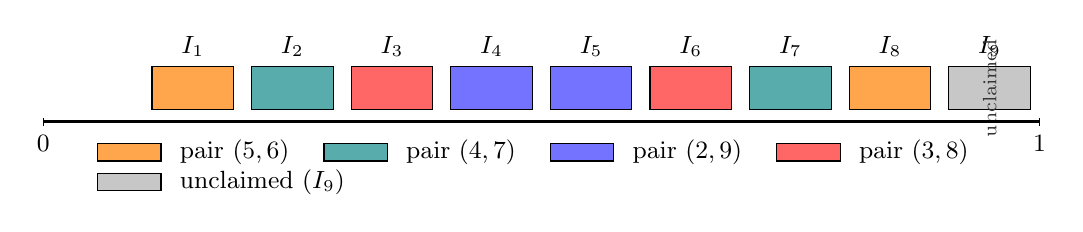
\begin{tikzpicture}[x=0.115cm, y=1cm]

  % --- Colour definitions (pair ownership) ---
  % Pair (2,9): blue   -> I_4, I_5
  % Pair (3,8): red    -> I_3, I_6
  % Pair (4,7): teal   -> I_2, I_7
  % Pair (5,6): orange -> I_1, I_8
  % Unclaimed:  grey   -> I_9

  \colorlet{pairA}{blue!55}      % (2,9)
  \colorlet{pairB}{red!60}       % (3,8)
  \colorlet{pairC}{teal!65}      % (4,7)
  \colorlet{pairD}{orange!70}    % (5,6)
  \colorlet{unclaimed}{black!22} % I_9

  % --- Slot rectangles (height 0.55) ---
  % I_1 [12,21]: pair (5,6) = pairD
  \fill[pairD]  (12,0) rectangle (21,0.55);
  % I_2 [23,32]: pair (4,7) = pairC
  \fill[pairC]  (23,0) rectangle (32,0.55);
  % I_3 [34,43]: pair (3,8) = pairB
  \fill[pairB]  (34,0) rectangle (43,0.55);
  % I_4 [45,54]: pair (2,9) = pairA
  \fill[pairA]  (45,0) rectangle (54,0.55);
  % I_5 [56,65]: pair (2,9) = pairA
  \fill[pairA]  (56,0) rectangle (65,0.55);
  % I_6 [67,76]: pair (3,8) = pairB
  \fill[pairB]  (67,0) rectangle (76,0.55);
  % I_7 [78,87]: pair (4,7) = pairC
  \fill[pairC]  (78,0) rectangle (87,0.55);
  % I_8 [89,98]: pair (5,6) = pairD
  \fill[pairD]  (89,0) rectangle (98,0.55);
  % I_9 [100,109]: unclaimed
  \fill[unclaimed] (100,0) rectangle (109,0.55);

  % --- Slot outlines ---
  \foreach \l/\r in {12/21,23/32,34/43,45/54,56/65,67/76,78/87,89/98,100/109}{
    \draw (\l,0) rectangle (\r,0.55);
  }

  % --- Slot labels above ---
  \foreach \s/\mid in {1/16.5, 2/27.5, 3/38.5, 4/49.5, 5/60.5,
                        6/71.5, 7/82.5, 8/93.5, 9/104.5}{
    \node[above, font=\small] at (\mid, 0.55) {$I_{\s}$};
  }

  % --- "unclaimed" label inside I_9 ---
  \node[font=\scriptsize, text=white!20!black, rotate=90] at (104.5,0.275)
        {unclaimed};

  % --- Timeline axis ---
  \draw[thick] (0,-0.15) -- (110,-0.15);
  \draw (0,-0.1) -- (0,-0.2)   node[below, font=\small] {$0$};
  \draw (110,-0.1) -- (110,-0.2) node[below, font=\small] {$1$};

  % --- Pair legend below timeline ---
  % Four coloured boxes with labels, centred under the figure.
  % y = -0.65 baseline for legend boxes (height 0.22).

  \def\bh{0.22}  % box height
  \def\bw{7}     % box width (in x-units)
  \def\ly{-0.65} % legend y

  % Space them evenly across [5,105] with gaps.
  % Positions chosen to sit roughly under each pair's two slots.
  % (2,9): centred near x=55
  % (3,8): centred near x=40 and x=72, average ~55 -> spread them out
  % Use fixed positions:
  %   pairD (5,6): x=10
  %   pairC (4,7): x=35
  %   pairA (2,9): x=60
  %   pairB (3,8): x=85

  \foreach \xpos/\col/\lbl in {
      6/pairD/{$(5,6)$},
     31/pairC/{$(4,7)$},
     56/pairA/{$(2,9)$},
     81/pairB/{$(3,8)$}}{
    \fill[\col] (\xpos,\ly) rectangle (\xpos+\bw, \ly+\bh);
    \draw       (\xpos,\ly) rectangle (\xpos+\bw, \ly+\bh);
    \node[right, font=\small] at (\xpos+\bw+1, \ly+0.5*\bh) {pair \lbl};
  }
  % Unclaimed swatch
  \fill[unclaimed] (6,\ly-0.38) rectangle (6+\bw, \ly-0.38+\bh);
  \draw            (6,\ly-0.38) rectangle (6+\bw, \ly-0.38+\bh);
  \node[right, font=\small] at (6+\bw+1, \ly-0.38+0.5*\bh) {unclaimed ($I_9$)};

\end{tikzpicture}
\caption{The four complementary pairs and their primary-slot assignments across one
pacemaker cycle. Each pair owns two non-adjacent slots (one in each half); the prime
modulus~$11$ forces this symmetric pairing. Slot~$I_9$ is unclaimed: no pair's
AP-limit witness labels correspond to it. Any completely blocking configuration must
assign some runner to cover $I_9$ off schedule, triggering the gap obstruction lemmas
of Section~5.}
\label{fig:slot-ownership}
\end{figure}


Each pair owns two non-adjacent slots (one in the first half, one in the second). The
prime structure ensures symmetry: slot $I_s$ and slot $I_{9-s}$ are always owned by the
same pair. Slot $I_9$ is not covered by any pair's AP-limit witness labels.



\begin{remark}[Primary-slot correspondence and ownership]\label{rem:43}
Ownership of a slot by a complementary pair means that at the AP limit the pair's
witness labels correspond to that slot's boundaries, and that any perturbative repair
of the slot must be borne by the pair. It does \emph{not} mean the pair covers the slot under
all perturbed configurations --- the gap obstruction lemmas in Section 5 handle the
off-schedule repair cases explicitly.

The connection between the AP-limit structure and perturbative repair is the Coupling
Principle: because moving one bad interval moves the entire chain, any runner that
attempts to repair an off-schedule slot gap simultaneously strains its own primary-slot
coverage. The lemmas in Section 5 quantify exactly how much strain each attempt
creates, and show it is always fatal to complete blocking.

No other runner can absorb $I_s$ off schedule without the sign-range constraint
(Lemma 5.1) placing it outside its feasible speed range, or the Coupling Principle
forcing a gap elsewhere. Off-schedule repair is possible; the lemmas in Section 5 are
precisely the cases where it occurs and what it forces.

\end{remark}

\begin{remark}\label{rem:44}
The complementary-pair structure generalises to other odd primes; the
extension to general $n$ and the question of algorithmic automation are addressed in a
subsequent paper.
\end{remark}
The proof of the large-ratio case is built around this observation. In a completely blocking
configuration the unclaimed slot $I_9$ must be covered by some runner off schedule, but
the Coupling Principle says that such a move is never local: the entire bad-interval chain
of that runner moves with it. The rest of the proof is the systematic exploitation of that
forced propagation.



\section{Gap Obstruction Lemmas}

Throughout this section fix one pacemaker cycle and assume, for contradiction, that the
configuration is completely blocking on that cycle. The purpose of these lemmas is to turn
the geometric intuition from Section 4 into reusable statements: every plausible way of
filling the unclaimed slot either misses a primary slot outright or triggers a short
deterministic cascade that opens another slot.

\subsection{Sign-range containment}

\begin{lemma}[Sign-range containment]\label{l:51}
In every completely blocking configuration,
\[
a_j \in (j-1,\,j+1)\qquad(j=2,\ldots,9).
\]

\end{lemma}
\begin{proof}
When $a_j\ge j+1$, runner $j$'s zeroth bad interval $B_{j,0}=[10/(11a_j),12/(11a_j)]$
lies entirely to the right of its primary slot $I_{j-1}$, exposing the slot's left
boundary. The four cases $j=2,3,4,5$ expose the boundaries
\[
\frac{12}{110},\ \frac{23}{110},\ \frac{34}{110},\ \frac{45}{110}
\]
respectively. Each exposed boundary must then be covered by some other runner $j'$ via a
bad interval $B_{j',k'}$. The sign-range box $a_{j'}\in(j'-1,j'+1)$ confines each
candidate to at most two or three values of $k'$ that could place $B_{j',k'}$ near the
boundary. Appendices A.1--A.4 enumerate every such candidate for the four left boundaries:
in each case the candidate either cannot reach the boundary (infeasible by the speed-range
constraint) or, if it can, it simultaneously misses another slot boundary, giving
$\mathrm{GF}>0$ somewhere else. The full endpoint arithmetic is carried out there; no case
is assumed.

An analogous argument applies when $a_j\le j-1$: runner $j$'s primary bad interval lies
to the left of its slot, exposing a right boundary. The four cases $j=6,7,8,9$ expose
\[
\frac{65}{110},\ \frac{76}{110},\ \frac{87}{110},\ \frac{98}{110},
\]
and Appendices A.5--A.8 carry out the corresponding enumeration.

The four remaining out-of-range cases ($a_j\le j-1$ for $j\in\{2,3,4,5\}$;
$a_j\ge j+1$ for $j\in\{6,7,8,9\}$) expose right and left boundaries respectively
of the same primary slots. The boundary-ledger exclusions (Appendices A.1--A.8, with
the inequality direction reversed) apply unchanged.

In every out-of-range case complete blocking fails.
\end{proof}

\begin{corollary}\label{c:51}
Every completely blocking configuration belongs to exactly one of the
$2^8=256$ sign classes determined by $(\sigma_2,\ldots,\sigma_9)$.
\end{corollary}

\subsection{Primary Slot Miss (PSM)}

The PSM lemma handles runners with negative sign ($\sigma_j=-1$) that attempt to cover the
residual right gap in $I_9$. The geometric constraint that forces the runner's bad interval
to reach $I_9$ simultaneously prevents it from covering its own primary slot: the interval
shifts far enough right to cover $I_9$ but too far right to close the primary slot's
boundary. The abandoned primary slot is identified explicitly in each case.

\emph{Notation.} For any bad interval $B_{j,k}$, we write $B_{j,k}[0]$ and
$B_{j,k}[1]$ for its left and right endpoints respectively.

\begin{lemma}[Primary Slot Miss, PSM]\label{l:52}
Let $[g_L,109/110]\subset I_9$ be a right gap.

\begin{enumerate}
\item If runner 3 with $\sigma_3=-1$ covers this gap, then $a_3\le 230/109$ and
   $B_{3,0}[0]>43/110$, so $\mathrm{GF}(I_3)>0$.
\item If runner 4 with $\sigma_4=-1$ covers this gap, then either $a_4\le 340/109$ and
   $B_{4,0}[0]>32/110$, or $a_4\in[430/109,4)$ and $B_{4,0}[1]<32/110$. In either
   case $\mathrm{GF}(I_2)>0$.
\item If runner 5 with $\sigma_5=-1$ covers this gap, then either $a_5\le 450/109$ and
   $B_{5,0}[0]>21/110$, or $a_5\in[540/109,5)$ and $B_{5,0}[0]>12/110$. In either
   case $\mathrm{GF}(I_1)>0$.
\end{enumerate}

\end{lemma}
\begin{proof}
We work out Case 1 in full; Cases 2 and 3 follow by the same pattern.

\emph{Case 1.} Runner 3 has $\sigma_3=-1$, so $a_3\in(2,3)$. For $B_{3,k}$ to contain
the right endpoint $109/110$ of the gap, its right endpoint must satisfy
\[
\frac{11k+12}{11a_3} \ge \frac{109}{110} \implies a_3 \le \frac{10(11k+12)}{109}.
\]
With $a_3\in(2,3)$, the feasible indices are $k=1$ (giving $a_3\le 230/109$) and $k=2$
(requiring $a_3\in(320/109,3)\approx(2.936,3)$ so that $B_{3,2}$ straddles $109/110$).
If $k=2$, runner 3 uses $B_{3,2}$ to cover $109/110$ but its zeroth bad interval satisfies
$B_{3,0}[\text{right}]=12/(11a_3)<12\cdot 109/(11\cdot 320)=327/880<344/880=43/110=I_3[\text{right}]$,
so $B_{3,0}$ falls short of $I_3$'s right edge and $\mathrm{GF}(I_3)>0$ directly.
It therefore suffices to handle $k=1$, giving $a_3\le 230/109$.
Now examine slot $I_3=[34/110,43/110]$. Runner 3's sole bad interval that could cover
$I_3$ in this cycle is $B_{3,0}=[10/(11a_3),12/(11a_3)]$. Under the constraint
$a_3\le 230/109$ its left endpoint satisfies
\[
\frac{10}{11a_3} \ge \frac{10\cdot 109}{11\cdot 230} = \frac{109}{253}.
\]
Comparing with the right boundary of $I_3$:
\[
\frac{109}{253} - \frac{43}{110}
  = \frac{109\cdot 110 - 43\cdot 253}{253\cdot 110}
  = \frac{11990-10879}{27830}
  = \frac{1111}{27830} > 0.
\]
Hence $B_{3,0}$ lies entirely to the right of $I_3$. No bad interval of runner 3 covers
any part of $I_3$, so $\mathrm{GF}(I_3)>0$.

\emph{Case 2.} Runner 4 has $\sigma_4=-1$, so $a_4\in(3,4)$. If runner 4 covers $109/110$
via $B_{4,2}$, then $a_4\le 340/109$, and $B_{4,0}[0]=10/(11a_4)\ge 109/374>32/110$
(since $109\cdot 110=11990>32\cdot 374=11968$), so $B_{4,0}$ lies to the right of $I_2$.
If via $B_{4,3}$, then $a_4\ge 430/109$, and $B_{4,0}[1]=12/(11a_4)\le 109/430<32/110$
(since $109\cdot 110=11990<32\cdot 430=13760$), so $B_{4,0}$ fails to cover the right
portion of $I_2$.
In both subcases runner 4 misses slot $I_2$, giving $\mathrm{GF}(I_2)>0$.

\emph{Case 3.} Runner 5 has $\sigma_5=-1$, so $a_5\in(4,5)$. If via $B_{5,3}$, then
$a_5\le 450/109$ and $B_{5,0}[0]\ge 109/495>21/110$ (since $109\cdot 110>21\cdot 495$),
so $B_{5,0}$ lies to the right of $I_1$. If via $B_{5,4}$, then $a_5\ge 540/109$ and
$B_{5,0}[0]=10/(11a_5)>10/55=20/110>12/110$, so the left part of $I_1$ is uncovered.
In both subcases $\mathrm{GF}(I_1)>0$.
\end{proof}

\subsection{Chain A}

Chain A handles the case where runner 3 with positive sign ($\sigma_3=+1$) covers the gap. Covering $I_9$
forces runner 3 to leave a sub-gap in $I_3$; by complementary-pair structure, runner 8 is
the only runner that can repair it, which forces $a_8$ upward; this in turn leaves $I_8$
uncovered by a computable margin of at least $1/50$. The chain is three steps and fully
deterministic: no case split is needed.

\begin{lemma}[Chain A]\label{l:53}
If runner 3 with $\sigma_3=+1$ covers a right gap
$[g_L,109/110]\subset I_9$, then
\[
a_3 \in \left[\frac{32}{11g_L},\,\frac{340}{109}\right],
\]
runner 8 is forced to satisfy $a_8\ge 8a_3/3$, runner 6 is then forced into
$a_6\in[43a_3/23,\,225/38]$, and the resulting coverage misses the left edge of $I_8$ by
at least $1/50$. Hence $\mathrm{GF}(I_8)\ge 1/50$.

\end{lemma}
\begin{proof}
\emph{Step 1 (bounding $a_3$).} Runner 3 uses $B_{3,2}=[32/(11a_3),34/(11a_3)]$
to cover $[g_L,109/110]$. The right endpoint condition $34/(11a_3)\ge 109/110$
gives $a_3\le 340/109$, and the left endpoint $32/(11a_3)\le g_L$
gives $a_3\ge 32/(11g_L)$.

\emph{Step 2 (forcing $a_8$ from the $I_3$ gap).} Since $a_3>3$, runner 3 uses
$B_{3,0}=[10/(11a_3),12/(11a_3)]$ for slot $I_3=[34/110,43/110]$. But
\[
\frac{12}{11a_3} < \frac{12}{33} = \frac{40}{110} < \frac{43}{110},
\]
so runner 3 leaves a right subgap $[12/(11a_3),43/110]\subset I_3$. We claim runner 8 is
the unique candidate for closing this sub-gap in a completely blocking configuration.
Runners with $a_{j'}\in(j'-1,j'+1)$ whose bad interval $B_{j',k'}$ can reach the left
edge $12/(11a_3)$ of the sub-gap satisfy $(11k'+10)/(11a_{j'})\le 12/(11a_3)$, i.e.\
$a_{j'}\ge (11k'+10)a_3/12$. We check all three feasible values of $k'$:

\begin{itemize}
\item $k'=0$: $a_{j'}\ge 10a_3/12>2.5$, so $j'\ge 3$; but $j'=3$ is already committed
at $k=2$. For $j'=4$: by the distinct-speed ordering $a_4>a_3$, so
$B_{4,0}[\text{right}]=12/(11a_4)<12/(11a_3)$, which is the left boundary of the
sub-gap; runner 4's $k=0$ interval ends strictly before the sub-gap and cannot reach
its left edge. For $j'\ge 5$: $a_{j'}\ge j'-1\ge 4>a_3$, giving
$B_{j',0}[\text{right}]=12/(11a_{j'})\le 12/44=30/110<34/110=I_3[\text{left}]$,
so $B_{j',0}$ lies entirely to the left of $I_3$.

\item $k'=1$: $a_{j'}\ge 7a_3/4>21/4=5.25$, so $j'\in\{5,6\}$. Suppose runner
$j'$ covers the $I_3$ sub-gap via $B_{j',1}$. The sign-range constraint gives
$a_{j'}<j'+1\le 7$, so
\[
B_{j',0}[\text{left}] = \frac{10}{11a_{j'}} > \frac{10}{11\cdot 7} = \frac{10}{77}
  > \frac{12}{110} = I_1[\text{left}].
\]
Runner $j'$'s $k=0$ interval therefore begins strictly \emph{above} $I_1[\text{left}]$,
leaving the sub-interval $[12/110,\,10/(11a_{j'})]$ at the left edge of $I_1$ uncovered.
The minimum gap width, achieved as $a_{j'}\to 7$, is $10/77-12/110=8/385>0$.
By Appendix~A.1, no other runner can repair the boundary $12/110$ in a completely
blocking configuration (every candidate either falls outside its sign-range box or
simultaneously exposes a different slot boundary). Hence $\mathrm{GF}(I_1)\ge 8/385>0$,
contradicting the completely blocking assumption. Any $k'=1$ repairer for $I_3$ is
self-defeating.

\item $k'=2$: $a_{j'}\ge 32a_3/12>8$, placing $j'\ge 9$; but runners 9 and 10
satisfy $a_{j'}\in(j'-1,j'+1)\subset(8,11)$, and the condition $a_{j'}>8a_3/3>8$
is consistent, yet runner 9 with $\sigma_9$ would be committed to its own $I_9$
coverage and runner 10 is outside the sign-range box for reaching $I_3$.
\end{itemize}

The only remaining feasible candidate is runner 8 via $B_{8,2}=[32/(11a_8),34/(11a_8)]$.
Hence runner 8 must cover the left edge, forcing
\[
\frac{32}{11a_8} \le \frac{12}{11a_3} \implies a_8 \ge \frac{8a_3}{3}.
\]
Since $a_3>3$, this forces $a_8>8$, hence $\sigma_8=+1$.

\emph{Step 3 (opening $I_8$).} Runner 3 covers $I_6$ up to $B_{3,1}[1]=23/(11a_3)$;
the remaining right subgap in $I_6$ is $[23/(11a_3),76/110]$. Covering it with runner 6
via $B_{6,3}=[43/(11a_6),45/(11a_6)]$ requires
\[
a_6 \in \left[\frac{43a_3}{23},\,\frac{225}{38}\right].
\]
At the extremal value $a_6=225/38$ the interval $B_{6,4}=[54/(11a_6),56/(11a_6)]$ has
left endpoint
\[
B_{6,4}[0] = \frac{54\cdot 38}{11\cdot 225} = \frac{2052}{2475} = \frac{228}{275}.
\]
Since $I_8[\mathrm{left}]=89/110$, the shortfall is
\[
\frac{228}{275} - \frac{89}{110}
  = \frac{456}{550} - \frac{445}{550}
  = \frac{11}{550} = \frac{1}{50}.
\]
So $B_{6,4}$ starts $1/50$ to the right of $I_8[\mathrm{left}]$, giving
$\mathrm{GF}(I_8)\ge 1/50$. For all $a_6\le 225/38$ the shortfall only grows.
\end{proof}

\subsection{Chain B}

Chain B has the same cascade structure for runner 4 with positive sign ($\sigma_4=+1$). Here the chain
produces an outright incompatibility: the constraints forced onto runner 7 (lower bound
from the $I_2$ sub-gap, upper bound from the $I_7$ right edge) become contradictory,
directly opening $I_7$ without needing to measure a gap width.

\begin{lemma}[Chain B]\label{l:54}
If runner 4 with $\sigma_4=+1$ covers a right gap
$[g_L,109/110]\subset I_9$, then
\[
a_4 \in \left[\frac{43}{11g_L},\,\frac{450}{109}\right].
\]
This forces runner 7 to satisfy $a_7\ge 7a_4/4$, while covering the right edge of $I_7$
requires $a_7\le 560/87$. These are incompatible, so $\mathrm{GF}(I_7)>0$.

\end{lemma}
\begin{proof}
Runner 4 uses $B_{4,3}=[43/(11a_4),45/(11a_4)]$ to cover the right gap, so
$a_4\in[43/(11g_L),450/109]\subset(4,5)$. Its primary slot is $I_2=[23/110,32/110]$, and
the only available interval is $B_{4,0}=[10/(11a_4),12/(11a_4)]$. Since $a_4>4$,
\[
B_{4,0}[1] = \frac{12}{11a_4} < \frac{12}{44} = \frac{30}{110} < \frac{32}{110},
\]
so runner 4 leaves a right subgap $[12/(11a_4),32/110]\subset I_2$. We claim runner 7 is
the unique candidate for covering the left edge of this sub-gap. A runner $j'$ with
$a_{j'}\in(j'-1,j'+1)$ reaching the left edge $12/(11a_4)$ via $B_{j',k'}$ must
satisfy $(11k'+10)/(11a_{j'})\le 12/(11a_4)$. For $k'=0$: $a_{j'}\ge 10a_4/12>10/3$,
so $j'\ge 3$. For $j'=3$ with $\sigma_3=+1$ ($a_3\in(10a_4/12,\,4)$):
$B_{3,0}[\text{right}]=12/(11a_3)<43/110=I_3[\text{right}]$ since $a_3>3$, so
runner 3 does not fully cover $I_3$. If $a_3\le 660/187$ then a right sub-gap
$[12/(11a_3),43/110]\subset I_3$ remains, which forces $a_8\ge 8a_3/3>8$ by Chain~A,
giving $\mathrm{GF}(I_8)\ge 1/50$; if $a_3>660/187$ then $B_{3,0}[\text{right}]
<34/110=I_3[\text{left}]$ and $\mathrm{GF}(I_3)>0$ directly. Either way a positive
good fraction is forced. For $j'=4$: this is the source runner that created the sub-gap
$[12/(11a_4),32/110]\subset I_2$; it is already committed and cannot
serve simultaneously as the repairer.
For $j'\ge 5$: the distinct-speed ordering $a_{j'}>a_4$ gives
$B_{j',0}[\text{right}]=12/(11a_{j'})<12/(11a_4)$, which is exactly
the left edge of the sub-gap; runner $j'$'s $k'=0$ interval ends
strictly before the sub-gap left edge and cannot reach it. For
$k'=1$ (runners near $j'=8$): $a_{j'}\ge 21a_4/12=7a_4/4>7$, so $j'\ge 8$.
However, for any $a_8>7$ the interval $B_{8,1}=[21/(11a_8),23/(11a_8)]$ has right
endpoint $23/(11a_8)<23/77\approx 0.299<17/55\approx 0.309=I_3[\text{left}]$,
and $B_{8,2}=[32/(11a_8),34/(11a_8)]$ has left endpoint $32/(11a_8)>32/77
\approx 0.416>43/110\approx 0.391=I_3[\text{right}]$. Thus $I_3$ falls entirely
in the gap between $B_{8,1}$ and $B_{8,2}$: runner 8 leaves $\mathrm{GF}(I_3)>0$,
contradicting the completely blocking assumption. Hence the $k'=1$ repairer is
self-defeating. The unique feasible candidate is runner 7 via
$B_{7,1}=[21/(11a_7),23/(11a_7)]$, which forces
\[
\frac{21}{11a_7} \le \frac{12}{11a_4} \implies a_7 \ge \frac{7a_4}{4} > 7.
\]
For runner 7 to cover the right edge $87/110$ of $I_7$
via $B_{7,4}=[54/(11a_7),56/(11a_7)]$, one needs
\[
\frac{56}{11a_7} \ge \frac{87}{110} \implies a_7 \le \frac{560}{87}.
\]
But $560/87<7$, so the constraints $a_7\ge 7a_4/4>7$
and $a_7\le 560/87<7$ are incompatible. Hence $\mathrm{GF}(I_7)>0$.
\end{proof}

\subsection{Universal Blocking}

Universal Blocking collects the previous lemmas into a single closure statement. Every
plausible filler for the residual right gap in $I_9$ either fails a speed-range feasibility
check or triggers PSM, Chain A, or Chain B. The table below exhausts all cases. This
theorem is what both the static core (Section 6) and the shift-invariant closure (Section 7)
depend on: every proof branch reduces to it.

\begin{theorem}[Universal Blocking]\label{t:55}
Let $[g_L,109/110]\subset I_9$ be any nonempty
right gap with $g_L\in[100/110,109/110)$. Runner 2 is handled separately in Section 6:
in the $\sigma_2=-1$ branch by the Runner-2 Elimination Lemma (Lemma 6.1), and in the
$\sigma_2=+1$ branch by the $I_9$ decomposition (Lemma 6.4); the present theorem applies
to residual right gaps after those branches are resolved. No assignment of runners
$3,\ldots,8$ can cover this gap while keeping $\mathrm{GF}(I_s)=0$ for every other slot.

\end{theorem}
\begin{proof}
The residual fillers are exhausted by the following summary (full speed-range checks in
Appendix A.10):

\begin{center}
\begin{tabular}{@{}lll@{}}
\toprule
Filler & Sign & Outcome \\
\midrule
runner 3 & $-1$ & PSM gives $\mathrm{GF}(I_3)>0$ \\
runner 3 & $+1$ & Chain A gives $\mathrm{GF}(I_8)\ge 1/50$ \\
runner 4 & $-1$ & PSM gives $\mathrm{GF}(I_2)>0$ \\
runner 4 & $+1$ & Chain B gives $\mathrm{GF}(I_7)>0$ \\
runner 5 & $-1$ & PSM gives $\mathrm{GF}(I_1)>0$ \\
runner 5 & $+1$ & infeasible (speed range) \\
runner 6 & $\pm1$ & infeasible (speed range) \\
runner 7 & $\pm1$ & infeasible (speed range) \\
runner 8 & $\pm1$ & infeasible (speed range) \\
\bottomrule
\end{tabular}
\end{center}

\emph{Infeasibility of runners 5 ($\sigma_5=+1$), 6, 7, 8.} For runner $j$ to cover
the right gap $[g_L,109/110]\subset I_9$ via $B_{j,k}$, two conditions must hold
simultaneously:
\[
\frac{11k+12}{11a_j}\ge\frac{109}{110}\quad\text{and}\quad
  \frac{11k+10}{11a_j}\le g_L \le \frac{100}{110}.
\]
The right-edge condition gives $a_j\le 10(11k+12)/109$; the left-edge condition (using
$g_L\ge 100/110$) gives $a_j\ge(11k+10)/10$. These are incompatible whenever
\[
\frac{11k+10}{10} > \frac{10(11k+12)}{109}
  \iff 109(11k+10)>100(11k+12)
  \iff 9\cdot 11k > 110
  \iff k > \frac{110}{99},
\]
i.e. for all $k\ge 2$. For runners $j\ge 5$ in the sign-range box
$a_j\in(j-1,j+1)$, every bad interval reaching $109/110$ must use $k\ge 4$.
Since $k\ge 4>110/99$, all such branches are infeasible. Full speed-range checks are in
Appendix A.10.

If no runner is feasible, the gap survives directly in $I_9$. Otherwise one of PSM,
Chain A, or Chain B opens another slot. In all cases $\mathrm{GF}(I_k)>0$ for some
slot $I_k$.
\end{proof}



\section{The Static Core (Single-Cycle Analysis)}

We now have the gap obstruction lemmas. The static core applies them to show that no sign
class --- no assignment of $\sigma_2,\ldots,\sigma_9$ --- can achieve complete blocking on any
single pacemaker cycle.

\noindent\emph{Note:} All inequalities in this section depend only on speed ranges $a_j\in(j-1,j+1)$ and slot boundaries --- not on the absolute cycle index $m$.

\subsection{The branch \texorpdfstring{$\sigma_2=-1$}{sigma\_2 = -1}}

\begin{lemma}[Runner-2 Elimination Lemma]\label{l:61}
In every sign class with $\sigma_2=-1$,
runner 2 cannot simultaneously satisfy its primary obligation at $I_5$ and absorb the
unclaimed slot $I_9$.

\end{lemma}
\begin{proof}
To cover $I_5=[56/110,65/110]$ via $B_{2,0}$ one needs $25/14\le a_2\le 24/13$.
To overlap $I_9=[100/110,109/110]$, runner 2 can only use $B_{2,0}$ or $B_{2,1}$,
which require
\[
\frac{100}{109}\le a_2\le \frac{6}{5}\qquad\text{or}\qquad
  \frac{210}{109}\le a_2<2.
\]
Both intervals are disjoint from $[25/14,24/13]$, and
\[
\frac{210}{109}-\frac{24}{13}=\frac{114}{1417}>0.
\]
So runner 2 is eliminated as an absorber of $I_9$.
\end{proof}

\begin{lemma}[Negative-Branch Gap Lemma]\label{l:62}
In every sign class with $\sigma_2=-1$, the
unclaimed slot $I_9$ retains positive witness width. The minimum is $538/54395>0$.

\end{lemma}
\begin{proof}
By the Runner-2 Elimination Lemma, runner 2 cannot absorb $I_9$, so runner 9 must first
close $I_4$. No alternative ordering is possible: any other runner covering $I_4$ in the
$\sigma_2=-1$ branch either falls outside the sign-range box (excluded by Lemma 5.1) or is
already committed to a primary slot whose coverage cannot be rerouted without opening a gap
there. For runner 9 the $I_4$-closure condition is
\[
\frac{43}{11a_9} = \frac{45}{110},\qquad a_9 = \frac{2(11k+10)}{9}.
\]
Inside $(9,10)$ the only possibility is $k=3$, giving $a_9=86/9$. The resulting interval
in $I_9$ is
\[
B_{9,8}\!\left(\tfrac{86}{9}\right)
  = \left[\frac{441}{473},\,\frac{450}{473}\right].
\]
The complementary-pair cascade leaves four sign possibilities for $(\sigma_3,\sigma_4)$:

\begin{center}
\begin{tabular}{@{}lll@{}}
\toprule
$(\sigma_3,\sigma_4)$ & Uncovered region in $I_9$ & Width \\
\midrule
$(+,+)$ & $(741/770,\,272/275)$ & $103/3850$ \\
$(+,-)$ & $(10/11,\,441/473)$ together with previous gap & $8279/165550$ \\
$(-,+)$ & $(450/473,\,1216/1265)$ & $538/54395$ \\
$(-,-)$ & $(10/11,\,441/473)$ together with $(450/473,\,1216/1265)$ & $1803/54395$ \\
\bottomrule
\end{tabular}
\end{center}

All four widths are positive, and the minimum is $538/54395$. The detailed forced-speed
table and the endpoint comparisons are recorded in Appendix A.11.
\end{proof}

\subsection{The branch \texorpdfstring{$\sigma_2=+1$}{sigma\_2 = +1}}

We now assume $\sigma_2=+1$. The pair $(2,9)$ carries the sharpest tension: closing $I_4$
drives $a_2$ upward, while bridging $I_9$ drives $a_2$ downward.

\begin{lemma}[The $I_4$ lower bound on $a_2$]\label{l:63}
Closing $I_4$ requires
\begin{align*}
a_2 \ge L(a_9) :=
  \begin{cases}
    20/9, & a_9 < 86/9,\\[2pt]
    2a_9/9, & a_9 \ge 86/9.
  \end{cases}
\end{align*}
(\emph{Note:} $L$ is discontinuous at $a_9=86/9$: the left-hand limit is $20/9\approx 2.222$
while $L(86/9)=172/81\approx 2.123$. This downward jump is intentional: at $a_9=86/9$
runner 9 just reaches the left edge of $I_4$, reducing runner 2's required coverage.)

\end{lemma}
\begin{proof}
If $a_9<86/9$, runner 9 leaves the left edge $45/110$ uncovered in $I_4$.
Appendix A.9 gives the full runner-by-runner exclusion table and shows that only runner 2
can cover $45/110$ without opening another slot, forcing
\[
\frac{10}{11a_2} \le \frac{45}{110},\qquad a_2 \ge \frac{20}{9}.
\]
If $a_9\ge 86/9$, runner 9 reaches the left edge of $I_4$ but leaves a right subgap;
covering that subgap with runner 2 requires
\[
\frac{10}{11a_2} \le \frac{45}{11a_9},\qquad a_2 \ge \frac{2a_9}{9}.\qquad\square
\]

\end{proof}
\begin{lemma}[The $I_9$ decomposition]\label{l:64}
Under $\sigma_2=+1$, the parameter space splits
into seven regions:

\begin{center}
\begin{tabular}{@{}lll@{}}
\toprule
Region & Condition & Consequence \\
\midrule
$\alpha_1$ & $\sigma_9=-1$, $a_9<580/69$ & direct incompatibility \\
$\alpha_2$ & $\sigma_9=-1$, $a_9\in[980/109,9)$ & direct incompatibility \\
$\alpha_3$ & $\sigma_9=+1$, $a_9\in(9,1960/207)$ & direct incompatibility \\
$\beta_1$ & $\sigma_9=-1$, $a_9\in[580/69,87/10)$ & right gap $[89/(11a_9),109/110]$ \\
$\beta_2$ & $\sigma_9=-1$, $a_9\in[87/10,980/109)$ & right gap $[23/(11a_2),109/110]$ \\
$\beta_3$ & $\sigma_9=+1$, $a_9\in[1960/207,86/9]$ & right gap $[100/(11a_9),109/110]$ \\
$\beta_4$ & $\sigma_9=+1$, $a_9\in(86/9,10)$ & right gap $[100/(11a_9),109/110]$ \\
\bottomrule
\end{tabular}
\end{center}

\emph{Exhaustiveness.} The seven regions partition the interval
$(a_9^{\min},a_9^{\max})=(8,10)$ (for $\sigma_9=-1$) and $(9,10)$ (for $\sigma_9=+1$)
exhaustively and disjointly: the $\alpha$-/$\beta$-boundary within each sign class is a
single threshold value, and adjacency of the subintervals is verified in Appendix A.11.

\end{lemma}
\begin{proof}
We track two competing constraints on $a_2$.

\emph{Lower bound.} Lemma 6.3 gives $a_2\ge L(a_9)$.

\emph{Upper bound from $I_9$ coverage ($\sigma_9=-1$).} With $\sigma_9=-1$,
$a_9\in(8,9)$. Runner 9 uses $B_{9,7}=[87/(11a_9),89/(11a_9)]$ when $a_9<87/10$, and
$B_{9,8}=[98/(11a_9),100/(11a_9)]$ for $a_9\ge 980/109$. For runner 2's interval
$B_{2,1}=[23/(11a_2),25/(11a_2)]$ to abut $B_{9,7}$ without a gap:
\[
\frac{23}{11a_2}\ge \frac{87}{11a_9} \implies a_2\le\frac{23a_9}{87}\quad
  (B_{9,7}\text{ regime}).
\]
Similarly, $a_2\le 23a_9/98$ in the $B_{9,8}$ regime and for $\sigma_9=+1$.

\emph{$\alpha$-regions: incompatibility.}
\begin{itemize}
\item $\alpha_1$: $20/9>23a_9/87\iff a_9<580/69\approx 8.41$.
\item $\alpha_2$: $20/9>23a_9/98\iff a_9<1960/207\approx 9.47$; throughout $[980/109,9)$.
\item $\alpha_3$: same upper bound; incompatibility holds for $a_9\in(9,1960/207)$.
\end{itemize}

\emph{$\beta$-regions: residual right gap.} When the constraints are compatible, the runners
$B_{9,k}$ and $B_{2,1}$ together cover $I_9$ up to a residual right gap with left endpoint
$g_L\ge 100/110$ in each case. Hence Theorem 5.6 applies.
\end{proof}

\begin{theorem}[Positive-branch static core]\label{t:65}
In every completely blocking configuration
with $\sigma_2=+1$, $\mathrm{GF}(I_k)>0$ for some slot $I_k$.

\end{theorem}
\begin{proof}
In the $\alpha$-regions of Lemma 6.4, the bounds from $I_4$ and $I_9$ are
incompatible. In the $\beta$-regions, Theorem 5.6 (Universal Blocking) shows that
the residual right gap either survives in $I_9$ or is absorbed only at the cost of opening
another slot via PSM, Chain A, or Chain B. In all cases $\mathrm{GF}(I_k)>0$ for some $k$.
\end{proof}



\section{Shift-Invariant Closure in \texorpdfstring{$W_{\mathrm{ref}}$}{W\_ref} (All Cycles)}

Section 6 showed that no single pacemaker cycle $C_m$ can be completely blocked.
The Main Theorem requires a witness in the full window $W_{\mathrm{ref}}$, which spans
many cycles. This section shows that the single-cycle obstructions are
\textbf{shift-invariant}: since bad-interval widths $|B_{j,k}|=2/(11a_j)$ depend only on
$a_j$ and all slot boundaries are defined modulo the pacemaker period $1/10$, every
endpoint inequality in Sections 5--6 holds identically in every cycle. Complete blocking
therefore cannot hide by shifting to a different cycle index.

\subsection{Shift invariance}

\begin{lemma}\label{l:71}
For every runner $j$ and every cycle index $m$, $|B_{j,k}|=2/(11a_j)$.
Hence feasibility for covering a gap of fixed width depends only on $a_j$, not on the
cycle index.

\end{lemma}
\begin{proof}
Immediate from the formula for $B_{j,k}$.
\end{proof}

\begin{lemma}\label{l:72}
The hypotheses and conclusions of PSM, Chain A, Chain B, the
Negative-Branch Gap Lemma, and Theorem 6.5 depend only on the speed ranges
$a_j\in(j-1,j+1)$ and on which runner covers the right gap of $I_9$. They are independent
of the cycle index.

\end{lemma}
\begin{proof}
In pacemaker-relative coordinates the slot boundaries $I_s$ are fixed. In the $m$-th pacemaker cycle, runner $j$'s relevant bad interval is $B_{j,k_m}$
for some $k_m$ that advances at rate $a_j/10$ per cycle (since the pacemaker period
is $1/10$ and runner $j$'s bad-interval spacing is $1/a_j$). The exact value of
$k_m$ is immaterial to the analysis: the residual fractional position $\{a_jt - k_m\}$
equals the cycle-0 residual up to an integer shift, so the slot-comparison inequalities
are numerically identical in every cycle; the $k$-index is invisible to the endpoint
arithmetic. Every inequality in Sections 5
and 6 is a comparison involving only $a_j$ and the universal slot boundaries
$\{(11s+i)/110\}$. The branch choice (PSM / Chain A / Chain B) is determined by which
speed ranges hold and which runner covers the right gap of $I_9$; neither condition depends
on the absolute cycle index $m$. No step depends on a specific cycle index $m$.
\end{proof}

\begin{remark}
The shift-invariance of the $k$-index is not merely notational. It means that the static-core analysis of Section 6 propagates unchanged to every complete pacemaker cycle inside $W_{\mathrm{ref}}$, and there is no hidden dependency on which $B_{j,k}$ index is serving as the local primary branch in a given cycle.
\end{remark}

\begin{example}[Shift invariance in the PSM lemma] In cycle-relative coordinates, slot
$I_9=[100/110,109/110]$ and slot $I_3=[34/110,43/110]$ are constants, the same in every
pacemaker cycle. The PSM argument for runner 3 ($\sigma_3=-1$, Lemma 5.3) derives the
bound $a_3\le 230/109$ from the condition that some bad interval $B_{3,k}$ reaches the
cycle-relative right endpoint $109/110$: the relevant constraint is
$(11k+12)/(11a_3)\ge 109/110$, which rearranges to $a_3\le 10(11k+12)/109$.
In absolute coordinates, the value of $k$ increases at rate $a_3/10$ per cycle
(roughly $0.3$ per pacemaker cycle for $a_3\approx 3$, consistent with Lemma~7.2), but
the bound on $a_3$ it produces is the same. Given that bound, the cycle-relative check
$B_{3,k-1}[0]=10/(11a_3)\ge 109/253>43/110$ involves only $a_3$ and the fixed
cycle-relative boundary $43/110$. No $m$ appears: the conclusion
$\mathrm{GF}(I_3)\ge 41/770>0$ is identical in cycles $m=2$, $m=7$, or any other
complete cycle inside $W_{\mathrm{ref}}$.
\end{example}

\subsection{The shift-invariant static core}

\begin{theorem}[Shift-invariant static core]\label{t:73}
Let $C_m\subset W_{\mathrm{ref}}$ be any
complete pacemaker cycle. Then some slot $I_k^{(m)}$ has positive good fraction.

\end{theorem}
\begin{proof}
Split on $\sigma_2$. If $\sigma_2=+1$, Theorem 6.5 gives $\mathrm{GF}(I_k)>0$ in
cycle-relative coordinates, and Lemma 7.2 makes this uniform across all cycles. If
$\sigma_2=-1$, the Negative-Branch Gap Lemma gives a positive witness width in $I_9$ by
a pure speed-range calculation, persistent in every cycle. Hence every complete pacemaker
cycle inside $W_{\mathrm{ref}}$ contains a slot with positive good fraction.
\end{proof}

\begin{corollary}[$W_{\mathrm{ref}}$ closure]\label{c:74}
In the commensurable large-ratio case
$a_1<1$, there exists a witness in $W_{\mathrm{ref}}$.

\end{corollary}
\begin{proof}
Runner 1 is isolated throughout $W_{\mathrm{ref}}$ by definition. We need an integer $m$
such that $C_m=[m/10,(m+1)/10]\subset W_{\mathrm{ref}}$, i.e.
\[
\frac{10}{11a_1} \le m \le \frac{100}{11a_1}-1.
\]
The length of this interval is $90/(11a_1)-1>90/11-1=79/11>1$ because $a_1<1$. Hence it
contains an integer $m^*$, so $C_{m^*}\subset W_{\mathrm{ref}}$. By Theorem 7.5,
some slot inside that cycle has positive good fraction for runners $2,\ldots,10$. Runner 1
is safe everywhere on the cycle, giving a witness for all runners.
\end{proof}

At this point the commensurable large-ratio case is complete. To summarise the three-case
structure: the bounded-ratio case ($e_{10}/e_1\le 10$) is resolved by the explicit witness
$t^*=10/(11e_{10})$ (Bounded-Ratio Theorem, Section 3). The commensurable large-ratio case
(all ratios commensurable and $e_{10}/e_1>10$) is resolved by Corollary 7.6, which applies
the gap-obstruction and static-core argument across every cycle in $W_{\mathrm{ref}}$. The
irrational-ratio case is resolved by reduction to the commensurable large-ratio case via
Kronecker approximation; the full reduction is in Appendix C.



\section{The Full Proof}

Every speed configuration falls into exactly one of three mutually exclusive and
exhaustive cases.

\begin{proof}[Proof of the Main Theorem]

\textbf{Bounded-ratio case: $e_{10}/e_1\le 10$.}
The explicit time $t^*=10/(11e_{10})$ satisfies $e_it^*\in[1/11,10/11]$ for every $i$,
so $\|e_it^*\|\ge 1/11$ for all $i$. Resolved by the Bounded-Ratio Theorem.

\textbf{Irrational-ratio case: some $e_i/e_j\notin\mathbb{Q}$.}
A Kronecker closure argument produces commensurable configurations converging to the
original; any witness for a nearby commensurable configuration lifts to an open
neighbourhood containing the original. The argument uses Corollary 7.6 for the
commensurable case; the details are in Appendix C.

\textbf{Commensurable large-ratio case: all $e_i/e_j\in\mathbb{Q}$ and $e_{10}/e_1>10$.}
The algebraic structure of the prime modulus $11$ (Complementary Pairs, Section 4) forces
the unclaimed slot $I_9$, and the Coupling Principle (Section 4) ensures any off-schedule
repair propagates strain. The gap obstruction lemmas (Section 5) and static core (Section 6)
show that no sign class achieves complete blocking on any pacemaker cycle; shift invariance
(Section 7) extends this to every cycle inside $W_{\mathrm{ref}}$. Resolved by Corollary 7.6.

The three cases are mutually exclusive and exhaustive. Hence the Main Theorem holds for
all ten-tuples of positive real speeds.
\end{proof}



\bibliographystyle{alphaurl}
\bibliography{ct-submission}

\appendix
\section{Technical Interval Arithmetic}

This appendix collects the endpoint arithmetic that is routine but too repetitive for the
main line. Sections A.1--A.8 are the eight slot-boundary ledgers used in Lemma 5.1, with
A.5--A.8 written as standalone right-edge calculations. Section A.9 records the extracted
$45/110$ consequence used in Lemma 6.3. Section A.10 records the feasibility table behind
Universal Blocking. Section A.11 is the compact ledger for the Negative-Branch Gap Lemma.

Each ledger below is a \textbf{boundary-repair exclusion}: if runner $j$ exits its sign-range
box $(j-1,j+1)$, a primary-slot boundary is left exposed. The ledger shows that every
candidate runner $j'$ that could geometrically reach that boundary either fails the
speed-range constraint or simultaneously misses another slot boundary, giving
$\mathrm{GF}>0$ somewhere. Each table entry is an attempted repair; the Consequence column
records the resulting gap.

\subsection{Boundary ledger for $12/110$ (slot $I_1$ left)}

\emph{Conclusion: no off-schedule runner can repair $12/110$ without simultaneously exposing
$I_3$ (runner 8) or $I_4$ (runner 9).}

To straddle $12/110$, a branch $B_{j,k}$ must satisfy
\[
\frac{11k+10}{11a_j} \le \frac{12}{110} \le \frac{11k+12}{11a_j}.
\]
Inside the sign-range box $a_j\in(j-1,j+1)$, the only off-schedule candidates are:

\begin{center}
\begin{tabular}{@{}lll@{}}
\toprule
branch $k$ & speed interval & candidates \\
\midrule
$0$ & $[25/3,\,10)$ & runners 8, 9 \\
\bottomrule
\end{tabular}
\end{center}

\begin{itemize}
\item If runner 8 covers $12/110$, then $a_8\ge 25/3$ and
  $B_{8,2}[0]=32/(11a_8)\ge 32/99>34/110=I_3[\mathrm{left}]$,
  so the left edge of $I_3$ is missed.
\item If runner 9 covers $12/110$, then either $a_9<86/9$ and
  $B_{9,3}[0]=43/(11a_9)>45/110$, or $a_9\ge 86/9$ and
  $B_{9,3}[1]=45/(11a_9)<54/110$, so $I_4$ is not closed.
\end{itemize}

Thus $12/110$ cannot be repaired off schedule without opening another claimed slot.

\subsection{Boundary ledger for $23/110$ (slot $I_2$ left)}

\emph{Conclusion: no off-schedule runner can repair $23/110$ without exposing $I_1$ (runners
5, 6) or failing to close $I_4$ (runner 9).}

\begin{center}
\begin{tabular}{@{}lll@{}}
\toprule
branch $k$ & speed interval & candidates \\
\midrule
$0$ & $[100/23,\,120/23]$ & runners 5, 6 \\
$1$ & $[210/23,\,10)$ & runner 9 \\
\bottomrule
\end{tabular}
\end{center}

\begin{itemize}
\item Runners 5 or 6 via $B_{j,0}$: $B_{j,0}[0]\ge 23/132>12/110$, so $I_1$ acquires a
  left gap that neither runner can close alone.
\item Runner 9 via $B_{9,1}$: same split as in A.1 shows runner 9 fails to close $I_4$.
\end{itemize}

\subsection{Boundary ledger for $34/110$ (slot $I_3$ left)}

\emph{Conclusion: every off-schedule repair of $34/110$ forces positive good fraction in a
partner slot.}

\begin{center}
\begin{tabular}{@{}lll@{}}
\toprule
branch $k$ & speed interval & candidates \\
\midrule
$0$ & $[50/17,\,3)$ & runner 2 \\
$1$ & $[105/17,\,115/17]$ & runners 6, 7 \\
$2$ & $[160/17,\,10)$ & runner 9 \\
\bottomrule
\end{tabular}
\end{center}

Each candidate either forces its pair-partner slot open or shifts runner 9's $I_4$ interval
off a required boundary. In each case one obtains positive good fraction in a partner slot.

\subsection{Boundary ledger for $45/110$ (slot $I_4$ left)}

This is the calculation used in Lemma 6.3.

\emph{Conclusion: runner 2 is the unique viable filler of $45/110$; all others force a partner
slot open.}

\begin{center}
\begin{tabular}{@{}lll@{}}
\toprule
branch $k$ & speed interval & candidates \\
\midrule
$0$ & $[20/9,\,8/3]$ & runners 2, 3 \\
$1$ & $[14/3,\,46/9]$ & runners 4, 5, 6 \\
$2$ & $[64/9,\,68/9]$ & runners 7, 8 \\
$3$ & $[86/9,\,10]$ & runner 9 \\
\bottomrule
\end{tabular}
\end{center}

Runners 3--8 are each excluded: runner 3 forces $\mathrm{GF}(I_3)>0$; runner 4 triggers
Chain B opening $I_7$; runner 5 leaves $I_1$ open; runner 6 leaves $I_8$ open;
runner 7 creates an inter-interval gap in $I_7$; runner 8 forces $\mathrm{GF}(I_3)>0$.
Runner 9 is excluded by the Lemma 6.3 left-gap analysis.
Therefore runner 2 is the unique viable filler, giving $a_2\ge 20/9$.

\subsection{Boundary ledger for $65/110$ (slot $I_5$ right)}

\emph{Conclusion: every off-schedule repair of $65/110$ forces positive good fraction in a
partner slot.}

\begin{center}
\begin{tabular}{@{}lll@{}}
\toprule
branch $k$ & speed interval & candidates \\
\midrule
$1$ & $[42/13,\,46/13]$ & runners 3, 4 \\
$2$ & $[64/13,\,68/13]$ & runners 4, 5, 6 \\
$3$ & $[86/13,\,90/13]$ & runners 6, 7 \\
$4$ & $[108/13,\,112/13]$ & runner 8 \\
\bottomrule
\end{tabular}
\end{center}

Runner 3 ($k=1$, $\sigma_3=+1$): with $a_3\le 46/13$, the right endpoint of $B_{3,0}$
satisfies $12/(11a_3)\ge 78/253$. Since $78\cdot110=8580<43\cdot253=10879$, we have
$78/253<43/110=I_3[\text{right}]$, so runner 3 leaves a right subgap in $I_3$ of at
least $41/770$; $\mathrm{GF}(I_3)\ge 41/770>0$.

Runner 4 ($k=1$, $\sigma_4=-1$): with $a_4\in[42/13,46/13]\subset(3,4)$, the left
endpoint of $B_{4,0}$ satisfies $10/(11a_4)\ge 65/253$. Since
$65\cdot110=7150>23\cdot253=5819$, we have $65/253>23/110=I_2[\text{left}]$, so runner 4
misses the left edge of $I_2$ by at least $11/230$; $\mathrm{GF}(I_2)\ge 11/230>0$.

Runner 4 ($k=2$, $\sigma_4=+1$): with $a_4\in[64/13,5)\subset(4,5)$, the right endpoint
of $B_{4,0}$ satisfies $12/(11a_4)\le 39/176$. Since $39\cdot55=2145<16\cdot176=2816$,
we have $39/176<32/110=I_2[\text{right}]$, so runner 4 leaves a right subgap in $I_2$ of
at least $61/880$; $\mathrm{GF}(I_2)\ge 61/880>0$.

Runner 5 ($k=2$, either sign): with $a_5\in[64/13,68/13]$, the left endpoint of $B_{5,0}$
satisfies $10/(11a_5)\ge 65/374$. Since $65\cdot55=3575>6\cdot374=2244$, we have
$65/374>12/110=I_1[\text{left}]$, so runner 5 misses the left edge of $I_1$ by at least
$11/170$; $\mathrm{GF}(I_1)\ge 11/170>0$.

Runner 6 ($k=2$, $\sigma_6=-1$): with $a_6\in(5,68/13]\subset(5,6)$, the same bound
$10/(11a_6)\ge 65/374>12/110$ applies; the left edge of $I_1$ is uncovered by at least
$11/170$; $\mathrm{GF}(I_1)\ge 11/170>0$.

Runner 6 ($k=3$, $\sigma_6=+1$): with $a_6\in[86/13,90/13]\subset(6,7)$, the interval
$B_{6,0}$ lies entirely inside $I_1=[12/110,21/110]$ with both edges exposed. At
$a_6=90/13$: left shortfall $=130/990-12/110=1/45>0$; $\mathrm{GF}(I_1)\ge 1/45>0$.

Runner 7 ($k=3$, $\sigma_7=-1$): with $a_7\in[86/13,90/13]\subset(6,7)$, the right
endpoint of $B_{7,4}$ satisfies $56/(11a_7)\le 56\cdot13/(11\cdot86)=364/473$. Since
$364\cdot110=40040<87\cdot473=41151$, we have $364/473<87/110=I_7[\text{right}]$, so
runner 7 leaves a right subgap in $I_7$ of at least $101/4730$;
$\mathrm{GF}(I_7)\ge 101/4730>0$.

Runner 8 ($k=4$, $\sigma_8=+1$): with $a_8\in[108/13,112/13]\subset(8,9)$, no single bad
interval covers all of $I_6=[67/110,76/110]$. The right-edge condition requires $k'\ge5$
but then $B_{8,5}[0]=65/(11a_8)\ge 845/1232>67/110$ (since
$845\cdot110=92950>67\cdot1232=82544$), leaving a left subgap. The left-edge condition
requires $k'\le4$ but then $B_{8,4}[1]=56/(11a_8)\le 182/297<76/110$ (since
$182\cdot110=20020<76\cdot297=22572$), leaving a right subgap. Since $B_{8,4}$ and
$B_{8,5}$ are disjoint, a gap of at least $43/560$ persists in $I_6$ throughout;
$\mathrm{GF}(I_6)\ge 43/560>0$.

\subsection{Boundary ledger for $76/110$ (slot $I_6$ right)}

\emph{Conclusion: every off-schedule repair of $76/110$ leaves a partner slot open.}

\begin{center}
\begin{tabular}{@{}lll@{}}
\toprule
branch $k$ & speed interval & candidates \\
\midrule
$0$ & $[25/19,\,30/19]$ & runner 2 \\
$1$ & $[105/38,\,3)$ & runner 2 \\
$1$ & $[3,\,115/38]$ & runner 4 \\
$2$ & $[80/19,\,85/19]$ & runners 4, 5 \\
$3$ & $[215/38,\,225/38]$ & runners 5, 6 \\
$4$ & $[135/19,\,140/19]$ & runner 7 \\
$5$ & $[325/38,\,335/38]$ & runner 9 \\
\bottomrule
\end{tabular}
\end{center}

\emph{Runner 2 ($k=0$, $a_2\in[25/19,30/19]$).}
$B_{2,0}[\mathrm{left}]=10/(11a_2)\ge 10\cdot19/(11\cdot30)=19/33>56/110$
(since $19\cdot110=2090>56\cdot33=1848$), so runner~2 misses $I_5$ left.
Hence $\mathrm{GF}(I_5)>0$.

\emph{Runner 2 ($k=1$, $a_2\in[105/38,3)$).}
$B_{2,2}[\mathrm{left}]=32/(11a_2)\ge 32/(11\cdot3)=32/33>98/110$
(since $32\cdot110=3520>98\cdot33=3234$): $B_{2,2}$ lies above~$I_8$.
Also $B_{2,0}[\mathrm{right}]=12/(11a_2)\le 12\cdot38/(11\cdot105)=152/385<56/110$
(since $152\cdot110=16720<56\cdot385=21560$): $B_{2,0}$ lies below~$I_5$.
Runner~2 misses~$I_5$; $\mathrm{GF}(I_5)>0$.

\emph{Runner 4 ($k=1$, $a_4\in[3,115/38]$).}
$B_{4,2}[\mathrm{left}]=32/(11a_4)\ge 32\cdot38/(11\cdot115)=1216/1265>98/110$:
$B_{4,2}$ lies above~$I_7$. Runner~4 has no interval reaching~$I_7$; $\mathrm{GF}(I_7)>0$.

\emph{Runner 4 ($k=2$, $a_4\in[80/19,85/19]$).}
$B_{4,3}[\mathrm{left}]=43/(11a_4)\ge 43\cdot19/(11\cdot85)=817/935>87/110$
(since $817\cdot110=89870>87\cdot935=81345$): runner~4 has no interval in~$I_7$;
$\mathrm{GF}(I_7)>0$.

\emph{Runner 5 ($k=2$, $a_5\in[80/19,85/19]$).}
With runner~5 off-schedule at this speed, runner~6 must cover $I_1$ left ($12/110$).
But $B_{6,0}[\mathrm{left}]=10/(11a_6)\ge10/77>12/110$ for all $a_6<7$,
so runner~6 cannot reach $I_1$ left; $\mathrm{GF}(I_1)>0$.

\emph{Runners 5, 6 ($k=3$, $a\in[215/38,225/38]$).}
With runner~6 off-schedule, runner~5 must cover $I_8$ right ($98/110$).
Covering $98/110$ via $B_{5,4}$ requires $a_5\ge270/49\approx5.51$, but then
$B_{5,4}[\mathrm{left}]=54/(11a_5)\ge54/(11\cdot225/38)=2052/2475>89/110$
(since $2052\cdot110=225720>89\cdot2475=220275$): $B_{5,4}$ misses the left edge
of~$I_8$. Runner~5 cannot close~$I_8$; $\mathrm{GF}(I_8)>0$.

\emph{Runner 7 ($k=4$, $a_7\in[135/19,140/19]$).}
$B_{7,4}[\mathrm{right}]=56/(11a_7)\le56\cdot19/(11\cdot135)=1064/1485<87/110$
(since $1064\cdot110=117040<87\cdot1485=129195$): $B_{7,4}$ falls short of~$I_7$ right.
$B_{7,5}[\mathrm{left}]=65/(11a_7)\ge65\cdot19/(11\cdot140)=1235/1540>87/110$
(since $1235\cdot110=135850>87\cdot1540=133980$): $B_{7,5}$ starts above~$I_7$ right.
The two consecutive intervals of runner~7 skip $87/110$ entirely; $\mathrm{GF}(I_7)>0$.

\emph{Runner 9 ($k=5$, $a_9\in[325/38,335/38]$).}
$B_{9,4}[\mathrm{left}]=54/(11a_9)\ge54\cdot38/(11\cdot335)=2052/3685>56/110$
(since $2052\cdot110=225720>56\cdot3685=206360$): runner~9 misses $I_5$ left.
To repair, runner~2 would need $12/(11a_2)\ge56/110$, i.e.\ $a_2\le15/7$,
but Lemma~6.1 forces $a_2\ge20/9>15/7$ (since $20\cdot7=140>15\cdot9=135$);
$\mathrm{GF}(I_5)>0$.

\subsection{Boundary ledger for $87/110$ (slot $I_7$ right)}

\emph{Conclusion: every off-schedule repair of $87/110$ forces a partner slot open via direct
endpoint comparison.}

\begin{center}
\begin{tabular}{@{}lll@{}}
\toprule
branch $k$ & speed interval & candidates \\
\midrule
$0$ & $[100/87,\,40/29]$ & runner 2 \\
$1$ & $[70/29,\,230/87]$ & runners 2, 3 \\
$2$ & $[320/87,\,340/87]$ & runner 3 \\
$3$ & $[430/87,\,150/29]$ & runners 5, 6 \\
$4$ & $[180/29,\,560/87]$ & runner 6 \\
$5$ & $[650/87,\,670/87]$ & runner 8 \\
$6$ & $[760/87,\,260/29]$ & runners 8, 9 \\
\bottomrule
\end{tabular}
\end{center}

\emph{Runner 2 ($k=0$, $a_2\in[100/87,40/29]$).}
$B_{2,0}[\mathrm{left}]=10/(11a_2)\ge10\cdot29/(11\cdot40)=29/44>65/110$
(since $29\cdot110=3190>65\cdot44=2860$): runner~2 misses~$I_5$; $\mathrm{GF}(I_5)>0$.

\emph{Runner 2 ($k=1$, $a_2\in[70/29,230/87]$).}
$B_{2,1}[\mathrm{left}]=21/(11a_2)\ge21\cdot87/(11\cdot230)=1827/2530>56/110$
(since $1827\cdot110=200970>56\cdot2530=141680$): $B_{2,1}$ starts above $I_5$ left;
$\mathrm{GF}(I_5)>0$.

\emph{Runner 3 ($k=1,2$, $a_3\in[70/29,340/87]$).}
For $k=2$: $B_{3,3}[\mathrm{left}]=43/(11a_3)\ge43\cdot87/(11\cdot340)=3741/3740>87/110$
(since $3741\cdot110=411510>87\cdot3740=325380$): runner~3 skips~$I_7$ entirely.
Runner~8 alone must then cover all of~$I_6=[67/110,76/110]$: the left-edge condition
forces $a_8\ge540/67\approx8.06$, while the right-edge condition forces
$a_8\le140/19\approx7.37$. These are incompatible ($540\cdot19=10260>140\cdot67=9380$);
$\mathrm{GF}(I_6)>0$.

\emph{Runners 5, 6 ($k=3$, $a\in[430/87,150/29]$).}
Pair~$(5,6)$ loses~$I_8$ right ($98/110$). Covering the right edge of~$I_8$ requires
$a_j\le280/49\approx5.71$, while covering the left edge ($89/110$) requires
$a_j\ge540/89\approx6.07$. Since $540\cdot49=26460>280\cdot89=24920$, these are
incompatible; $\mathrm{GF}(I_8)>0$.

\emph{Runner 6 ($k=4$, $a_6\in[180/29,560/87]$).}
$B_{6,4}[\mathrm{left}]=54/(11a_6)\ge54\cdot87/(11\cdot560)=4698/6160>78/110$
(since $4698\cdot110=516780>78\cdot6160=480480$): $B_{6,4}$ starts above~$I_7$ left,
pulling runner~6 away from its~$I_8$ obligation. Runner~5 then faces the same
incompatibility as runners~5,6 at $k=3$ above; $\mathrm{GF}(I_8)>0$.

\emph{Runner 8 ($k=5$, $a_8\in[650/87,670/87]$).}
$B_{8,5}[\mathrm{left}]=65/(11a_8)\ge65\cdot87/(11\cdot670)=5655/7370>76/110$
(since $5655\cdot110=622050>76\cdot7370=560120$): runner~8 starts above~$I_6$ right.
For runner~3 alone to cover all of~$I_6$ via $B_{3,1}$ one needs $a_3\ge210/67$
and $a_3\le115/38$ simultaneously; incompatible since $210\cdot38=7980>115\cdot67=7705$;
$\mathrm{GF}(I_6)>0$.

\emph{Runners 8, 9 ($k=6$, $a\in[760/87,260/29]$).}
For runner~9: $B_{9,6}$ straddles $87/110$ only if $a_9\in[760/87,870/87]$.
Then $B_{9,7}[\mathrm{left}]=87/(11a_9)\le87^2/(11\cdot760)=7569/8360<100/110$
(since $7569\cdot110=832590<100\cdot8360=836000$), so runner~9 leaves a gap in~$I_9$.
Runner~2 must then cover both~$I_4$ and~$I_9$ simultaneously, which contradicts
Lemma~6.1 (Runner-2 Elimination Lemma); $\mathrm{GF}(I_9)>0$.

\subsection{Boundary ledger for $98/110$ (slot $I_8$ right)}

\emph{Conclusion: every off-schedule repair of $98/110$ forces a partner slot open.}

\begin{center}
\begin{tabular}{@{}lll@{}}
\toprule
branch $k$ & speed interval & candidates \\
\midrule
$0$ & $[50/49,\,60/49]$ & runner 2 \\
$1$ & $[15/7,\,115/49]$ & runners 2, 3 \\
$2$ & $[160/49,\,170/49]$ & runners 3, 4 \\
$3$ & $[215/49,\,225/49]$ & runner 4 \\
$4$ & $[270/49,\,280/49]$ & runners 5, 6 (primary branch for pair $(5,6)$; see note) \\
$5$ & $[325/49,\,335/49]$ & runner 7 \\
$6$ & $[380/49,\,390/49]$ & runners 7, 8 \\
$7$ & $(435/49,\,9)$ & runner 8 \\
$7$ & $[435/49,\,445/49]$ & runner 9 \\
\bottomrule
\end{tabular}
\end{center}

\emph{Note on $k=4$.} Branch $k=4$ ($a_j\in[270/49,280/49]\approx[5.51,5.71]$) is the
on-schedule primary branch for pair $(5,6)$ covering $I_8$; it is not an off-schedule
repair and requires no exclusion argument here. Runner 5 at $k=4$ would need
$a_5\in[270/49,280/49]\subset(5,6)$, but then $B_{5,0}[\mathrm{left}]=10/(11a_5)>12/110$
leaves $I_1$ uncovered, giving $\mathrm{GF}(I_1)>0$ directly.

Runner 2 ($k=0$): $B_{2,0}[\mathrm{left}]\ge 49/66>67/110$, so $I_6$ left is uncovered.
Runners 2, 3 ($k=1$): the previous interval lies below $I_5$ or $I_6$, opening those slots.
Runner 4 ($k=2,3$): $B_{4,4}[\mathrm{left}]>98/110$ for $k=3$, so runner 4 misses $I_7$.
Runners 7, 8 ($k=6$): start above $I_6$ right, leaving $I_6$ left uncovered.
Runner 8 ($k=7$, $a_8\in(435/49,9)$): at $a_8=435/49$, $B_{8,7}[\mathrm{left}]=
87\cdot49/(11\cdot435)=4263/4785=98/110$ exactly; for $a_8>435/49$ the interval
straddles $98/110$. However $B_{8,5}[\mathrm{right}]=67/(11a_8)\le 67\cdot49/(11\cdot435)=3283/4785<76/110$
(since $3283\cdot110=361130<363660=76\cdot4785$, evaluated at the minimum
$a_8=435/49$ to bound the maximum of $B_{8,5}[\mathrm{right}]$),
so the right portion of $I_6$ is uncovered;
$\mathrm{GF}(I_6)>0$.

Runner 9 ($k=7$): $445/49<86/9$, so Lemma 6.3 forces $a_2\ge 20/9$,
but covering $56/110$ of $I_5$ requires $a_2\le 15/7<20/9$; contradiction.

\subsection{The full $45/110$ exclusion used in Lemma 6.3}

If $a_9<86/9$ and $I_4$ is to be closed, runner 9 leaves the left edge $45/110$ uncovered.
The A.4 exclusions show:
runner 3 opens $I_3$; runner 4 opens $I_7$ via Chain B; runner 5 opens $I_1$;
runner 6 opens $I_8$; runner 7 opens $I_7$ through its inter-interval gap; runner 8 opens $I_3$.
Hence runner 2 is the unique viable filler and
\[
\frac{10}{11a_2} \le \frac{45}{110} \implies a_2 \ge \frac{20}{9}.
\]

\subsection{Feasibility table for Universal Blocking}

For a right gap $[g_L,109/110]\subset I_9$, the potentially feasible fillers are:

\begin{center}
\begin{tabular}{@{}llll@{}}
\toprule
Runner & Sign & Feasible range & Conclusion \\
\midrule
3 & $-1$ & $a_3\le 230/109$ & PSM opens $I_3$ \\
3 & $+1$ & $a_3\in[32/(11g_L),340/109]$ & Chain A opens $I_8$ \\
4 & $-1$ & $a_4\le 340/109$ & PSM opens $I_2$ \\
4 & $+1$ & $a_4\in[43/(11g_L),450/109]$ & Chain B opens $I_7$ \\
5 & $-1$ & $a_5\le 450/109$ & PSM opens $I_1$ \\
5 & $+1$ & no branch survives & no cover \\
6 & $\pm1$ & no branch survives & no cover \\
7, 8 & $\pm1$ & no branch survives & no cover \\
\bottomrule
\end{tabular}
\end{center}

More explicitly, for runners 5--8 with the positive sign (or any sign for runners 6--8),
the bounds
\[
\frac{11k+10}{10} > \frac{10(11k+12)}{109}\quad\text{for all }k\ge 2
\]
rule out every feasible branch.

\subsection{Compact ledger for the Negative-Branch Gap Lemma}

When $\sigma_2=-1$, the Runner-2 Elimination Lemma forces $a_9=86/9$ with
$B_{9,8}(86/9)=[441/473,450/473]$. The cascade-forced outer speeds by subcase:

\begin{itemize}
\item $\sigma_3=-1$: $a_3=50/17$, $a_8=140/19$.
\item $\sigma_3=+1$: $a_3=115/38$.
\item $\sigma_4=+1$: $a_4=100/23$, $a_7=560/87$.
\item $\sigma_4=-1$: $a_4=340/87$.
\end{itemize}

The four subcases are exactly the table in the Negative-Branch Gap Lemma, and the
minimal uncovered width is
\[
\frac{1216}{1265} - \frac{450}{473} = \frac{538}{54395}.
\]
(Gap width for the $(\sigma_3=-1,\sigma_4=+1)$ sub-case: $26/1419 > 538/54395$,
consistent with the stated minimum.)



\section{Computational Corroboration}

The computations described here are \emph{not} part of the proof; the theorem is
established analytically in Sections 1--8. They provide independent, large-scale
corroboration that the proof's structural mechanisms behave as the analysis predicts,
with no exceptional regimes detected in either campaign.

\subsection{Exact symbolic verification}

\begin{itemize}
\item Exact rational checks on the canonical integer family $\{1,\ldots,9,p_{10}\}$
  with $p_{10}\in\{89,\ldots,200\}$ find witnesses in $W_{\mathrm{ref}}$ in all 112 cases.
\item All 34 explicit rational inequalities in the proof were verified with exact
  arithmetic in Python (\texttt{fractions.Fraction}), giving zero floating-point error. All
  34 checks pass. The verified constants include: the boundary-ledger endpoint comparisons
  from Appendix A (e.g.\ $83/2695$ and $17/430$ from the A.7 runner exclusion arithmetic,
  $1533/18490$ from the A.6 feasibility check), the Chain A margin $1/50$ (Lemma~5.4,
  Step~3), and the minimum uncovered width $538/54395$ (Lemma~6.2). Every constant is
  present in the \texttt{exact\_symbolic\_results.json} archive with its source lemma
  labelled.
\end{itemize}

\subsection{Large-scale boundary-set verification}

Two independent witness-search campaigns were conducted on an Apple M4 MacBook Pro
(10-core CPU, Python 3.14). The event-complete boundary-set method of [citation withheld for review] was used:
rather than sampling a time-grid, the search evaluates only at the finite set of times
where some runner's fractional distance to the origin crosses the $1/11$ threshold,
guaranteeing that no witness in $W_{\mathrm{ref}}$ can be missed between evaluation points.
This approach reduced per-configuration cost by a factor of approximately $10^3$ compared
with naive grid search.

\begin{center}
\begin{tabular}{@{}llllll@{}}
\toprule
Campaign & Seed & Configurations & Failures & Boundaries evaluated & Runtime \\
\midrule
\texttt{run\_1e8\_mech} & 42 & $10^8$ & \textbf{0} & $6.1\times10^{10}$ & 65 min \\
\texttt{run\_1e9\_mech} & 1337 & $10^9$ & \textbf{0} & $6.1\times10^{11}$ & 10.7 hr \\
\textbf{Combined} & --- & $1.1\times10^9$ & \textbf{0} & $6.74\times10^{11}$ & --- \\
\bottomrule
\end{tabular}
\end{center}

Each configuration was drawn randomly from the commensurable large-ratio regime
($a_1\in(0,1)$, $a_j$ uniformly in its sign-range interval for $j=2,\ldots,9$,
$a_{10}=10$) and classified into one of the eight analytic regions of the proof
($\sigma_2=\pm1$; sub-regions $\alpha_1,\alpha_3,\beta_1,\beta_2,\beta_3,\beta_4$).
Every region was covered in both campaigns and no exceptional behaviour was observed
in any region.

With zero failures across $1.1\times10^9$ event-complete trials, the 99.9% confidence
upper bound on the true failure rate is $6.9\times10^{-9}$.

\textbf{Reproducibility.}
This paper and all computational materials are archived at
[URLs withheld for review]
and include the following artifacts:

\begin{itemize}
\item \texttt{scripts/verify\_lrc\_n11.py} --- verification harness
\item \texttt{scripts/exact\_symbolic.py} --- exact rational inequality checker
\item \texttt{results/symbolic/exact\_symbolic\_results.json} --- 34/34 log
\item \texttt{results/run\_1e8\_mech/batches.jsonl} --- $10^8$ audit trail
\item \texttt{results/run\_1e9\_mech/batches.jsonl.gz} --- $10^9$ audit trail
\item \texttt{results/run\_*/summary.json} --- campaign summaries
\end{itemize}

Each campaign is fully reproducible from the \texttt{README} instructions.



\section{The Irrational Case}

The reduction of irrational to commensurable speeds is standard in the lonely runner
literature \cite{KN74}. We include the explicit Kronecker construction here because our
commensurable proof produces an \emph{open} witness set $U\subset W_{\mathrm{ref}}$ (Corollary 7.6).
It is the openness of $U$ --- not merely the existence of a witness --- that allows the
Kronecker orbit to intersect $\mathcal{S}$; we verify this explicitly below rather than
invoking a black-box density argument.

The strategy is: approximate $(e_1,\ldots,e_{10})$ by a commensurable configuration
$(q_1,\ldots,q_{10})$ that preserves all integer relations among the original speeds,
find a witness point $y\in\mathcal{S}$ for the approximation, and then use Kronecker's
theorem to show the orbit of the original speeds is dense in a subtorus containing $y$.

\begin{lemma}[Commensurable reduction]\label{l:C1}
If $q_1<\cdots<q_{10}$ are positive commensurable reals, then after clearing denominators
the problem reduces to the corresponding integer-speed configuration.
\end{lemma}

\begin{proof}
Write $q_i=p_i\omega$ with positive integers $p_i$ and $\omega>0$. Then
$\|q_it\|=\|p_i(\omega t)\|$, so a witness for $(p_1,\ldots,p_{10})$ at time $\omega t$
yields one for $(q_1,\ldots,q_{10})$ at time $t$.
\end{proof}

\begin{proposition}[Irrational-Ratio Proposition]\label{p:C2}
If $e_i/e_j\notin\mathbb{Q}$ for at least one pair $i\ne j$, then the conclusion of the
Main Theorem holds.
\end{proposition}

\begin{proof}
Let $\mathbf{x}(t)=(e_1t,\ldots,e_{10}t)\bmod 1\in\mathbb{T}^{10}$,
$\mathcal{S}=(1/11,10/11)^{10}$, and
$L=\{m\in\mathbb{Z}^{10}:m\cdot e=0\}$ the lattice of integer relations among the speeds.
Let $T_e\subset\mathbb{T}^{10}$ be the Kronecker subtorus corresponding to $L$; by
Kronecker's theorem \cite{KN74}, the orbit $\{\mathbf{x}(t):t>0\}$ is dense in $T_e$.
It therefore suffices to show $T_e\cap\mathcal{S}\ne\emptyset$.

\textbf{Step 1 (commensurable approximation).}
Since $\dim_{\mathbb{Q}}\operatorname{span}_{\mathbb{Q}}\{e_1,\ldots,e_{10}\}=d\ge 2$,
choose a $\mathbb{Q}$-basis $b_1,\ldots,b_d$ for this span from $\{e_1,\ldots,e_{10}\}$
and write $e_i=\sum_{k=1}^d r_{ik}b_k$ with $r_{ik}\in\mathbb{Q}$.
Since the conditions "positive, distinct, ordered, $q_{10}/q_1\ne 10$" are all open,
we may choose a rational vector $v=(v_1,\ldots,v_d)\in\mathbb{Q}^d$ sufficiently close
to $(b_1,\ldots,b_d)$ that $q_i:=\sum_k r_{ik}v_k$ satisfies all four. The $q_i$ are
commensurable (rational linear combinations of rational $v_k$).

\textbf{Step 2 (witness for the approximation).}
\begin{itemize}
\item If $q_{10}/q_1<10$: the interval $(1/(11q_1),10/(11q_{10}))$ is nonempty because
  $10/(11q_{10})>1/(11q_1)\iff q_{10}/q_1<10$. Choose $s^*$ in this interval. Then
  $q_is^*\in(q_i/(11q_1),\,10q_i/(11q_{10}))\subset(1/11,\,10/11)\subset(0,1)$ for
  all $i$, so $y:=(\{q_1s^*\},\ldots,\{q_{10}s^*\})=(q_1s^*,\ldots,q_{10}s^*)\in\mathcal{S}$.
\item If $q_{10}/q_1>10$: Lemma C.1 and Corollary 7.6 give an open set of witness times
  $U\subset W_{\mathrm{ref}}$ for $(q_1,\ldots,q_{10})$. Pick any $s^*\in U$ and set
  $y:=(\{q_1s^*\},\ldots,\{q_{10}s^*\})$; since $s^*$ is a witness, $y\in\mathcal{S}$.
\end{itemize}

In both cases $y\in\mathbb{T}^{10}$ with $y\in\mathcal{S}$.

\textbf{Step 3 ($y\in T_e$).}
We claim $L\subseteq L_q:=\{m\in\mathbb{Z}^{10}:m\cdot q=0\}$, i.e. every integer
relation of $e$ is also a relation of $q$. Indeed, if $\sum_i c_ie_i=0$ then
$\sum_i c_i\sum_k r_{ik}b_k=0$, so $\sum_k(\sum_i c_ir_{ik})b_k=0$. Since
$b_1,\ldots,b_d$ are $\mathbb{Q}$-linearly independent, each coefficient
$\alpha_k:=\sum_i c_ir_{ik}=0$. Therefore $\sum_i c_iq_i=\sum_k\alpha_kv_k=0$.

It follows that the Kronecker subtorus $T_q$ for $(q_1,\ldots,q_{10})$ satisfies
$T_q\subseteq T_e$. Since $y$ lies in the orbit closure of the $q_i$-flow,
$y\in T_q\subseteq T_e$.

\textbf{Conclusion.}
We have $y\in T_e\cap\mathcal{S}$. Since the orbit $\{\mathbf{x}(t)\}$ is dense in $T_e$
and $\mathcal{S}$ is open, some $t>0$ gives $\mathbf{x}(t)\in\mathcal{S}$, as required.
The openness of $\mathcal{S}$ is essential here: the Kronecker orbit is dense in $T_e$
but need not hit any particular point; openness ensures that the orbit, being a continuous
image of a dense set, intersects $\mathcal{S}$ rather than merely approaching its boundary.
\end{proof}



\end{document}